\documentclass[11pt, oneside]{book}

\usepackage[spanish]{babel}
\usepackage[utf8x]{inputenc}
%\usepackage[TS1, T1]{fontenc}
\usepackage[x11names]{xcolor}
\usepackage{pdfpages}
%\usepackage{fourier}
\usepackage{array, booktabs, url, caption, graphicx, epstopdf, colortbl}
\DeclareCaptionFont{blue}{\color{LightSteelBlue3}}

\newcommand{\foo}{\color{LightSteelBlue3}\makebox[0pt]{\textbullet}\hskip-0.5pt\vrule width 1pt\hspace{\labelsep}}

\begin{document}
  \setcounter{page}{0}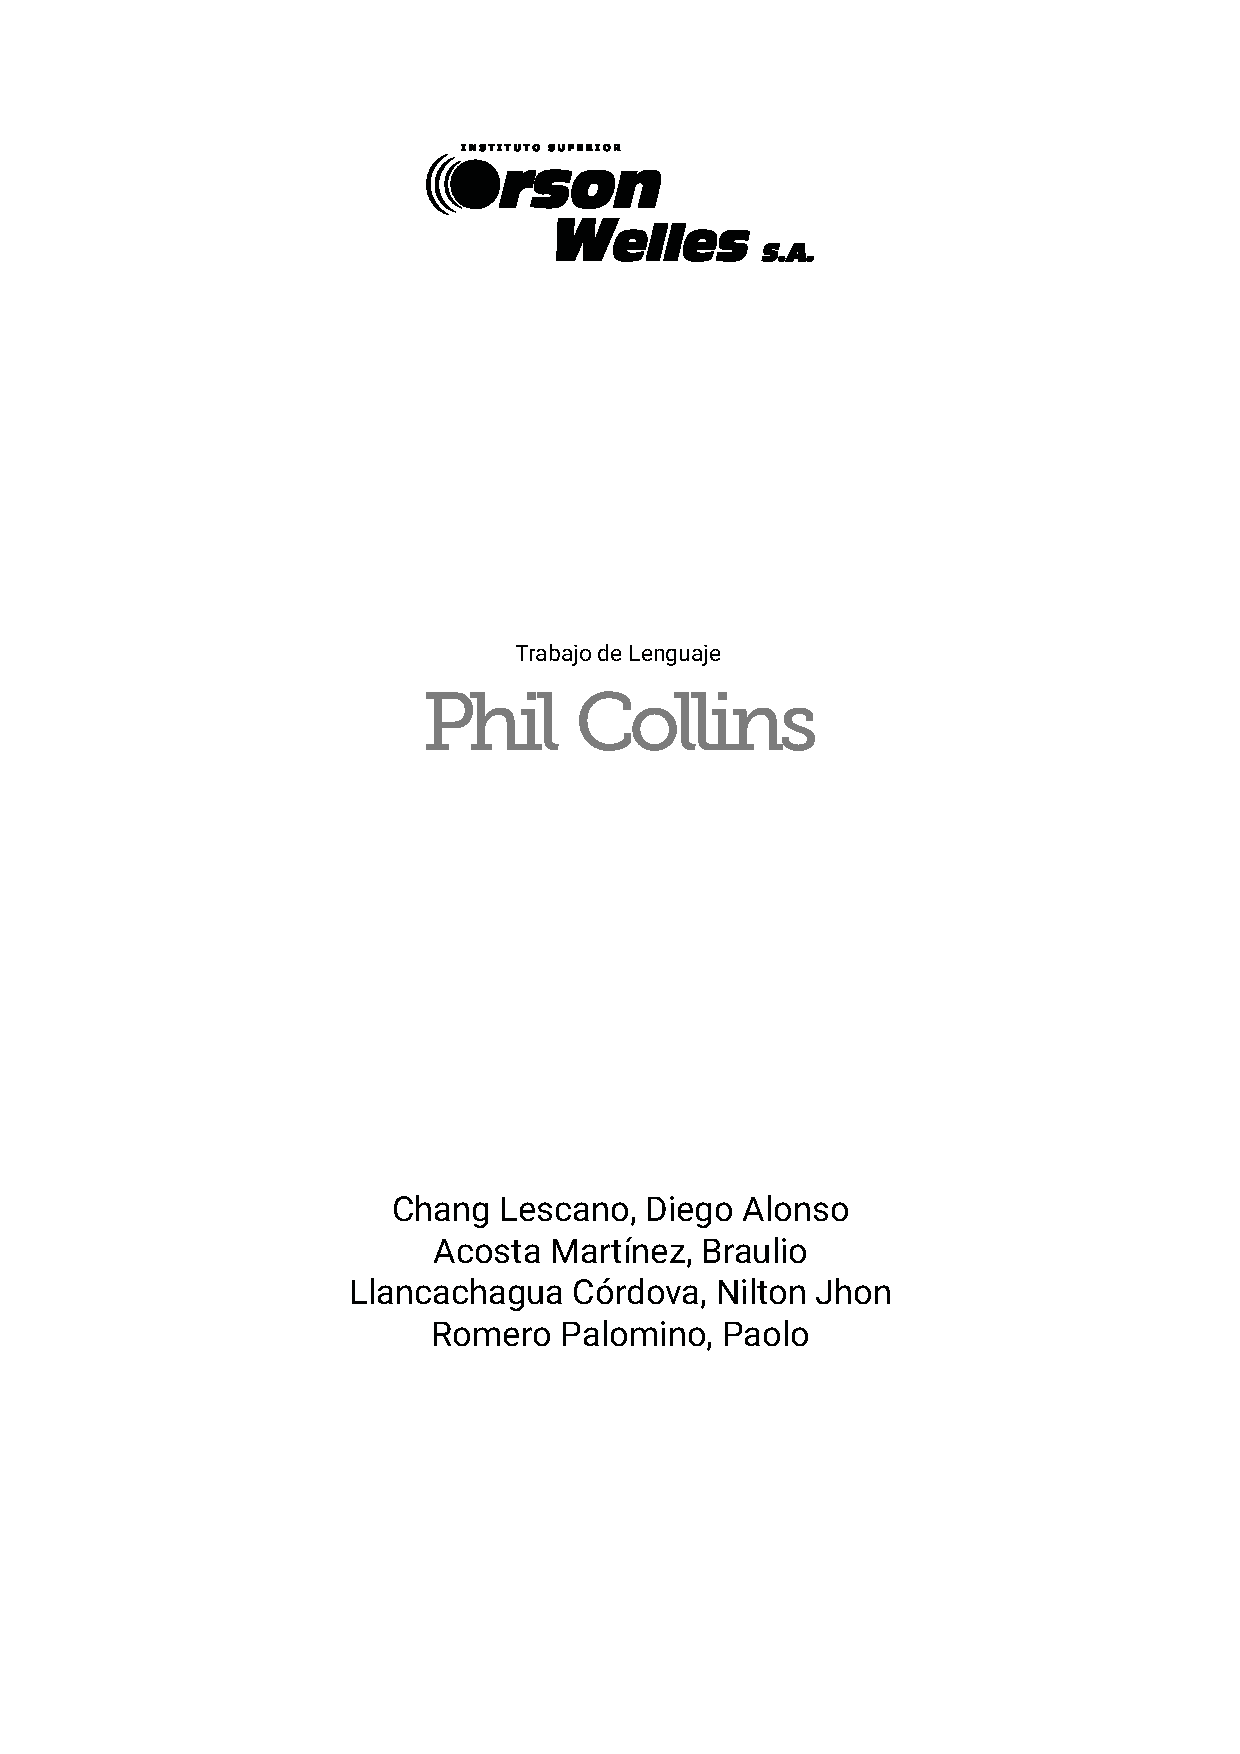
\includepdf{portada}

  \tableofcontents
  
  \chapter*{Introducción}
  \addcontentsline{toc}{chapter}{Introducción}

  Reconocido como uno de los artistas que ayudó a sentar las bases de la música de la época junto a su banda Genesis, Phil Collins ha llegado a convertirse en una megaestrella después de componer temás para películas animadas tan populares como \emph{Tarzan} (1999), y haber puesto varias canciones suyas en la punta de las listas musicales alrededor del planeta.\\

  Con este trabajo se intenta averiguar un poco sobre la carrera musical de este gran música, así como los problemas por los que ha tenido que pasar para realizar su música; y las razones para que haya decidido dejar la escena musical.\\

  Esto, por que alguna vez regrese a la misma.

  \chapter{Biografía}

  \begin{figure}
    \begin{center}
      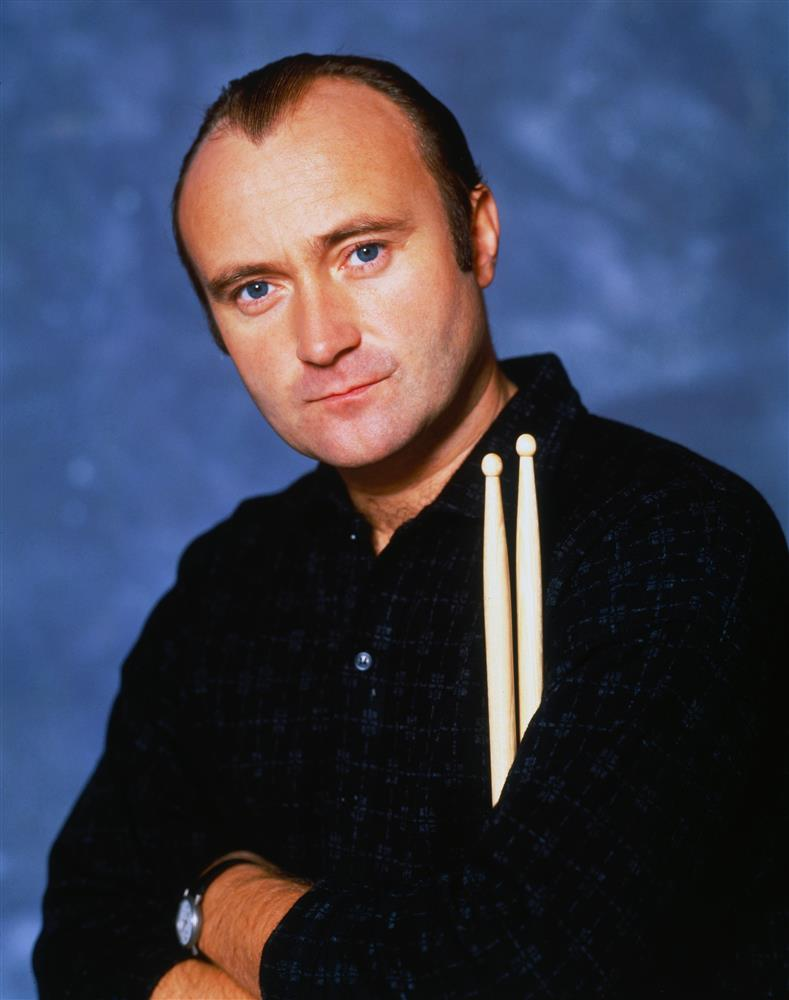
\includegraphics[scale = 0.6]{img/01.jpg}
    \end{center}
    \caption*{Phil Collins, baterista de la banda Genesis y compositor solista.}
  \end{figure}

  Philip David Charles Collins, o más conocido como Phil Collins, nació el 30 de enero de 1951 en el condado histórico de Middlesex,  Inglaterra. Su padre Greville Collins era agente de seguros y su madre Winifred era una manager teatral. El interés por la música de Phil nace a la edad de cinco años cuando sus padres le regalan por navidad una batería de juguete \cite{WIKI}.\\

  A los catorce años entro en la escuela de artes Barbara Speake Stage School. Empezó a trabajar como actor y modelo, ganando su primer papel importante como Artful Dodger en la producción de Oliver!. Participaría también en la película de \emph{The Beatles' A Hard Day's Night} y en \emph{Chitty Chitty Bang Bang}.\\

  A pesar de los inicios de su carrera como actor, Collins comenzó a orientarse hacia la música, formó una banda llamada The Real Thing más tarde se unió a The Freehold. Con este último grupo escribió su primera canción, titulada ``Lying Crying Dying''.\\

  La primera grabación de Phil fue como baterista del grupo Flaming Youth en el disco titulado \emph{Ark 2} (1969). Después de un año de gira, las tensiones dentro de la banda y la falta de éxito comercial terminaron por disolver el grupo.\\

  En 1970 Collins acude a la audición de la banda Genesis, donde se buscaba un batería sensible a la música acústica, y un guitarrista de acústica de doce cuerdas. La audición consistió en tocar algunas pistas del segundo álbum del grupo, \emph{Trespass} (1970). Como Collins llegó temprano, pudo memorizar las piezas escuchando a los demás.\\

  Un año después el grupo sacaría al mercado su tercer álbum, \emph{Nursery Cryme}, donde Phil Collins se encargaría de la batería, la percusión y los coros, y lo continuaría haciendo en los cinco años siguientes, a través de LPs clásicos del grupo como \emph{Foxtrot} (1972), o \emph{Selling England by the Pound} (1973).\\

  \begin{figure}
    \begin{center}
      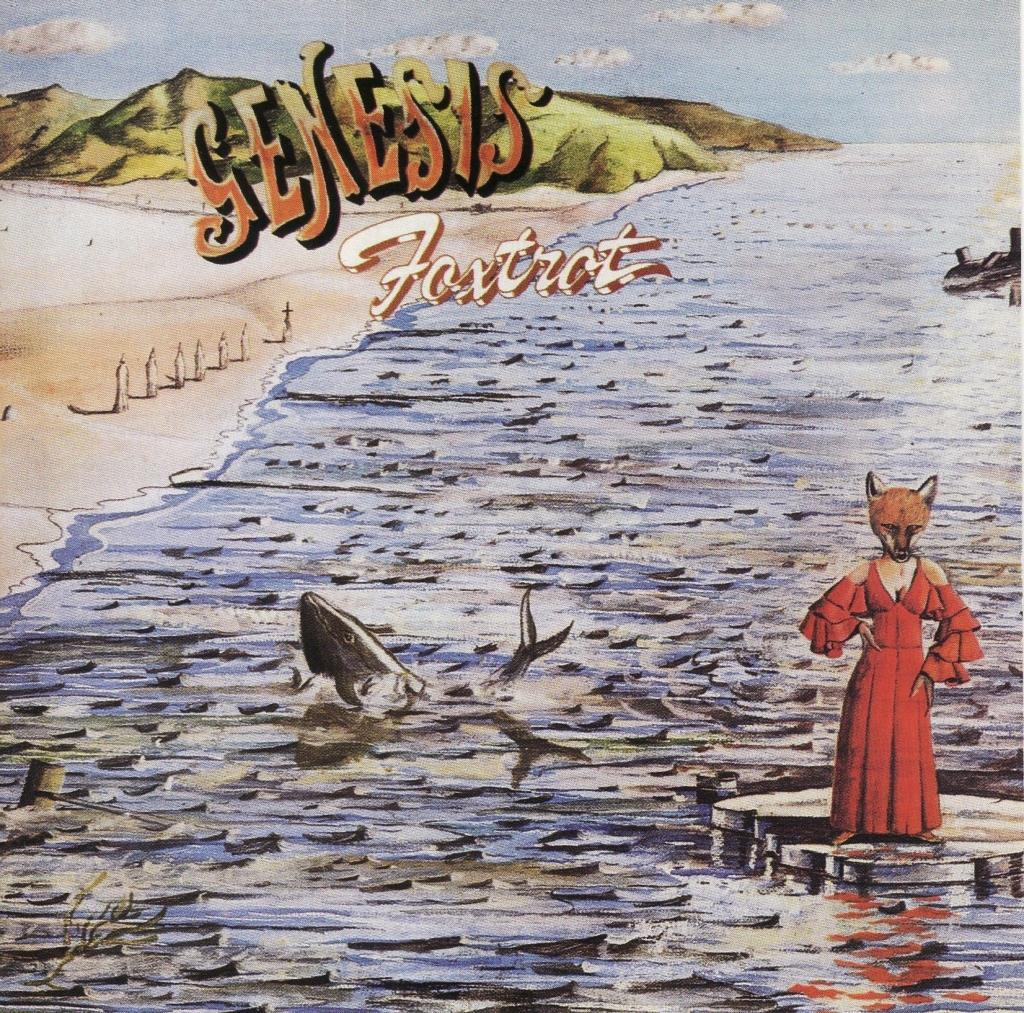
\includegraphics[scale = 0.4]{img/02.jpg}
    \end{center}
    \caption*{Portada del álbum \emph{Foxtrot}, lanzado en 1972 mientras que Peter Gabriel todavía estaba en Genesis.}
  \end{figure}

  En 1975, tras la gira final del álbum \emph{The Lamb Lies Down on Broadway}, Peter Gabriel abandona el grupo. Collins se convirtió en la voz principal hasta encontrar el reemplazo de Gabriel. En el corto plazo, el grupo contrató a Bill Bruford para tocar también la batería durante las presentaciones en vivo, aunque Collins continuó desempeñando su rol de instrumentalista en la banda durante las grabaciones. Pronto Bruford fue reemplazado por Chester Thompson. En este año se casó con la canadiense Andrea Bertorelli. Se conocieron como estudiantes en una clase de teatro en Londres. Tuvieron un hijo, Simon Collins, y Phil adoptó a la hija de Bertorelli, Joely Collins, que hoy día es una actriz canadiense.\\

  El primer álbum de esa nueva etapa fue \emph{A Trick of the Tail} (1976), que alcanzó al tercer puesto en las listas del Reino Unido y el Top 40 en Estados Unidos. La revista Rolling Stone, confirmó: ``Genesis ha conseguido convertir la posible catástrofe de la partida de Gabriel en su primer éxito estadounidense''.\\

  Steve Hackett se separa del grupo para iniciar su carrera como solista en 1977; el grupo quedó reducido a un trío, con Phil Collins haciéndose cargo de las voces, Mike Rutherford de guitarras y bajo (en estudio) y Tony Banks en teclados y voces, a formación regular incluía al baterista Chester Thompson y al guitarrista estadounidense Daryl Stuermer para los conciertos en vivo. La música de Genesis vería un cambio al pasar del rock progresivo al pop rock. Cabe destacar que esta última es la alineación con más éxito comercial.\\

  En los años ochenta, mientras Collins desarrollaba su carrera con Genesis, estableció una paralela como solista. Con el grupo Genesis grabó una serie de exitosos álbumes entre 1980 y 1986, incluyendo \emph{Duke}, \emph{Abacab}, \emph{Genesis} e \emph{Invisible Touch}.\\

  Collins graba su primer álbum, \emph{Face Value}, 9 de febrero de 1981, los asuntos predominantes en las letras de su álbum estaban relacionados con la ruptura de su primer matrimonio, y su entonces reciente divorcio. Hizo su debut en vivo como artista solista en el concierto a beneficio de Amnistía Internacional, \emph{The Secret Policeman's Other Ball} en el Theatre Royal de Londres en setiembre del mismo año.\\

  \emph{Face Value} se convirtió en un sorpresivo éxito internacional encabezando las listas en al menos siete países, alcanzando el top 10 del Billboard 200, y consiguiendo eventualmente un triple-platino en Estados Unidos.\\

  El 1 de noviembre de 1982 lanza su segundo álbum \emph{Hello, I Must Be Going!}, que fue número uno en el Reino Unido por su versión del tema de The Supremes ``You Can't Hurry Love''.\\

  En 1984 se casa con su segunda esposa, Jill Tavelman, ese mismo año lanzó la balada, ``Against All Odds (Take a Look at Me Now)'', que fue el tema principal de la película del mismo nombre, el cual se convirtió en el primer sencillo del músico en llegar al número uno del \emph{Billboard Hot 100} y se ganó la nominación al Óscar como mejor canción.\\

  Collins gana su primer Grammy en la categoría Mejor interpretación vocal pop masculina por su canción ``Against All Odds (Take a Look at Me Now)''.\\

  A comienzos de 1985, Collins lanzó su álbum más exitoso denominado \emph{No Jacket Required} el cual ha vendido más de 25 millones de copias. Contiene los éxitos número uno ``Sussudio'', ``One More Night'', así como ``Don't Lose My Number'' y ``Take Me Home''. \emph{No Jacket Required} pasó a ganar varios premios Grammy por mejor álbum del año.\\

  En 1989 nace su hija Lily Jane Collins de su segundo matrimonio, el 20 de noviembre Collins lanzó otro exitoso álbum en solitario, \emph{\dots But Seriously}, el cual incluía el himno ``Another Day in Paradise'', con David Crosby en los coros. ``Another Day in Paradise'' fue número 1 en las listas de Billboard a finales de 1989 y Collins ganó un Premio Brit al mejor sencillo británico en el año 1990 y el Premio Grammy en 1991 por mejor grabación del año. \emph{\dots But Seriously} se convirtió en el primer álbum \#1 en los Estados Unidos de la década de 1990 con aproximadamente 20 millones de copias.\\

  En 1991, Genesis, luego de seis años, saca otro disco \emph{We Can't Dance}, el cual sería el último álbum de estudio de Phil Collins con la banda.\\

  El record de ventas de Collins empezó a descender luego de la publicación de su disco Both Sides en 1993, un álbum en gran medida experimental donde Collins no utilizo músicos de apoyo y todas las piezas vocales e instrumentos lo realiza en su estudio casero.\\

  En 1996 Collins se separa de su segunda esposa, Jill Tavelman, y también oficialmente de Genesis para centrarse en su carrera como solista. Intentó regresar a la música pop con su disco \emph{Dance Into the Light}. Aunque el álbum obtuvo un disco de oro en los Estados Unidos, sus ventas fueron considerablemente menores que sus álbumes anteriores. A pesar de ello, la gira posterior mantuvo las entradas agotadas.\\

  Collins formó The Phil Collins Big Band, tocando él mismo la batería, la banda realizó diversos hits tanto de Genesis como de Phil en solitario, en versiones jazz. La Big Band de Phil Collins llevó a cabo una gira mundial en 1998.\\

  Hizo un álbum recopilatorio llamado Hits editado en 1998 y también grabo ``You'll Be in My Heart'', single para la película animada de Disney Tarzán. El tema gano un Globo de Oro y un Óscar a la mejor canción en 1999 y el 16 de junio fue galardonado con una estrella en el Paseo de la fama de Hollywood.\\

  Phil Collins se casó con su tercera esposa, Orianne Cevey, en 1999 tras un romance de cinco años. Tienen dos hijos, Nicholas y Matthew.\\

  En el 2002 lanzó \emph{Testify}, su séptimo álbum de estudio como solista, el cual fue elaborado a lo largo de dos años en su casa de Suiza. Fue fríamente recibido en EE.UU. e Inglaterra, aunque obtuvo cierto suceso en Europa continental, mientras que la gira de promoción, \emph{First Final Farewell Tour}, resultó ser exitosa.\\

  En 2006, y tras muchas especulaciones Collins se reunió con Mike Rutherford y Tony Banks, reactivando Genesis para la gira \emph{Turn It On Again: The Tour}, la cual fue anunciada el 7 de noviembre de ese año. La gira tuvo lugar durante el verano de 2007, y abarcó 12 países de Europa, extendiéndose luego a Norteamérica\\

  Collins y su esposa anunciaron su separación el 16 de marzo de 2006 y se divorciaron el 17 de agosto de 2008. Collins pagó presuntamente a Cevey £25M en acuerdo.\\

  Luego de varios años de inactividad regresó al panorama discográfico con un nuevo disco que vio la luz en septiembre de 2010 llamado \emph{Going Back} en el cual Collins reversionó temas clásicos del estilo R\&B y soul característico del sello Motown.\\

  \chapter{Discografía}
  \begin{figure}
    \begin{center}
      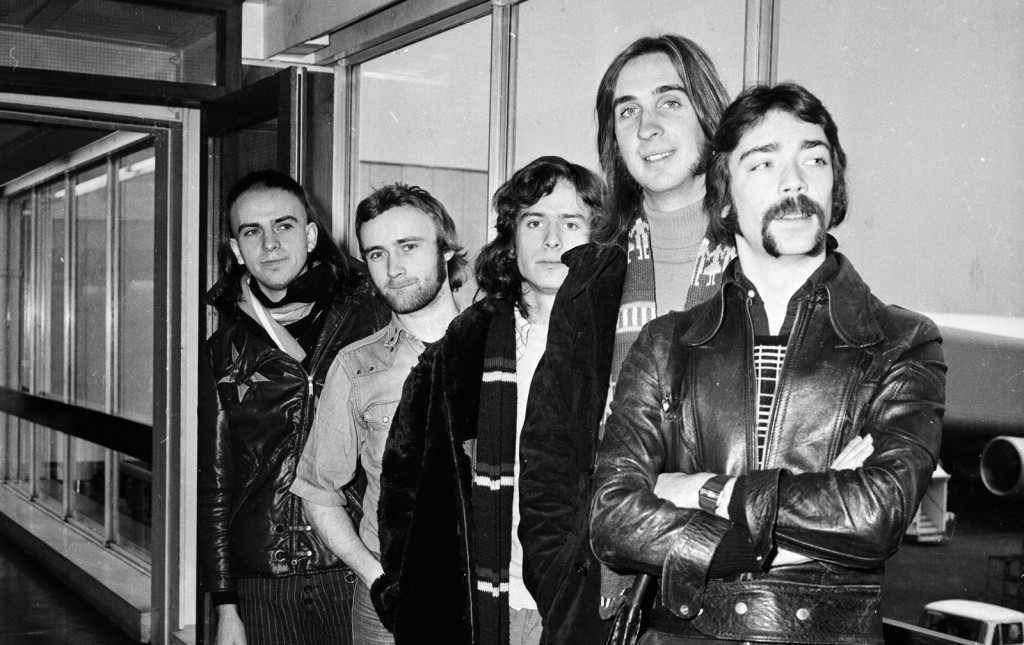
\includegraphics[scale = 0.4]{img/03.jpg}
    \end{center}
    \caption*{La banda Genesis \emph{circa} 1972.}
  \end{figure}

  Phil Collins grabó un total de 11 álbumes de estudio con la banda Genesis, y en 7 de estos fue la voz principal de la banda. Como solita, llegó a grabar 8 álbumes, sin contar los álbumes en vivo y una que otra banda sonora que llegó a realizar mientras estaba activo como músico

  \begin{table}
  \renewcommand\arraystretch{1.4}\arrayrulecolor{LightSteelBlue3}
  \captionsetup{singlelinecheck=false, font=blue, labelfont=sc, labelsep=quad}
  \caption{Discografía de Genesis con Phil Collins}\vskip -1.5ex
    \begin{tabular}{@{\,}r <{\hskip 2pt} !{\foo} >{\raggedright\arraybackslash}p{5cm}}
    \toprule
    \addlinespace[1.5ex]
      1971 & \emph{Nursery Cryme}\\
      1972 & \emph{Foxtrot}\\
      1973 & \emph{Selling England by The Pound}\\
      1974 & \emph{The Lamb Lies Down on Broadway}\\
      1976 & \emph{A Trick of the Tail}\\
      1978 & \emph{Wind \& Wuthering}\\
      1980 & \emph{\dots And Then There Were Three\dots}\\
      1981 & \emph{Duke}\\
      1983 & \emph{Abacab}\\
      1986 & \emph{Genesis}\\
      1991 & \emph{Invisible Touch}
    \end{tabular}
  \end{table}

  \begin{table}
  \renewcommand\arraystretch{1.4}\arrayrulecolor{LightSteelBlue3}
  \captionsetup{singlelinecheck=false, font=blue, labelfont=sc, labelsep=quad}
  \caption{Discografía de Phil Collins como solista}\vskip -1.5ex
    \begin{tabular}{@{\,}r <{\hskip 2pt} !{\foo} >{\raggedright\arraybackslash}p{5cm}}
    \toprule
    \addlinespace[1.5ex]
      1981 & \emph{Face Value}\\
      1982 & \emph{Hello, I Must Be Going!}\\
      1985 & \emph{No Jacket Required}\\
      1989 & \emph{\dots But Seriously}\\
      1993 & \emph{Both Sides}\\
      1996 & \emph{Dance into the Light}\\
      2002 & \emph{Testify}\\
      2010 & \emph{Going Back}
    \end{tabular}
  \end{table}

  \chapter{Un momento difícil}

  En 2011 se hizo anunció que Phil iba a dar un pazo al costado del mundo musical por problemas relacionados a la batería. Más adelante se revela que los problemas estaban relacionados con la audición, una vértebra dislocada y daño en los nervios de las manos en consecuencia por haber tocado la batería por tantos años.

  \begin{quotation}
    No estoy preocupado por no ser capaz de tocar batería de nuevo; estoy más preocupado por ser capaz de cortar un pedazo de pan seguramente y construir cosas para mis hijos. \cite{enfermo}
  \end{quotation}

  El asunto no fue discutido por mucho tiempo, pero, al respecto, se dijo que lso problemas llegaron cuando una lesión al cuello le produjo daños a los nervios de las manos, lo que le impide sostener las baquetas con la fuerza necesaria. Antes había mencionado que él necesitaba pegarse las baquetas a las manos para poder tocar.

  \begin{figure}
    \begin{center}
      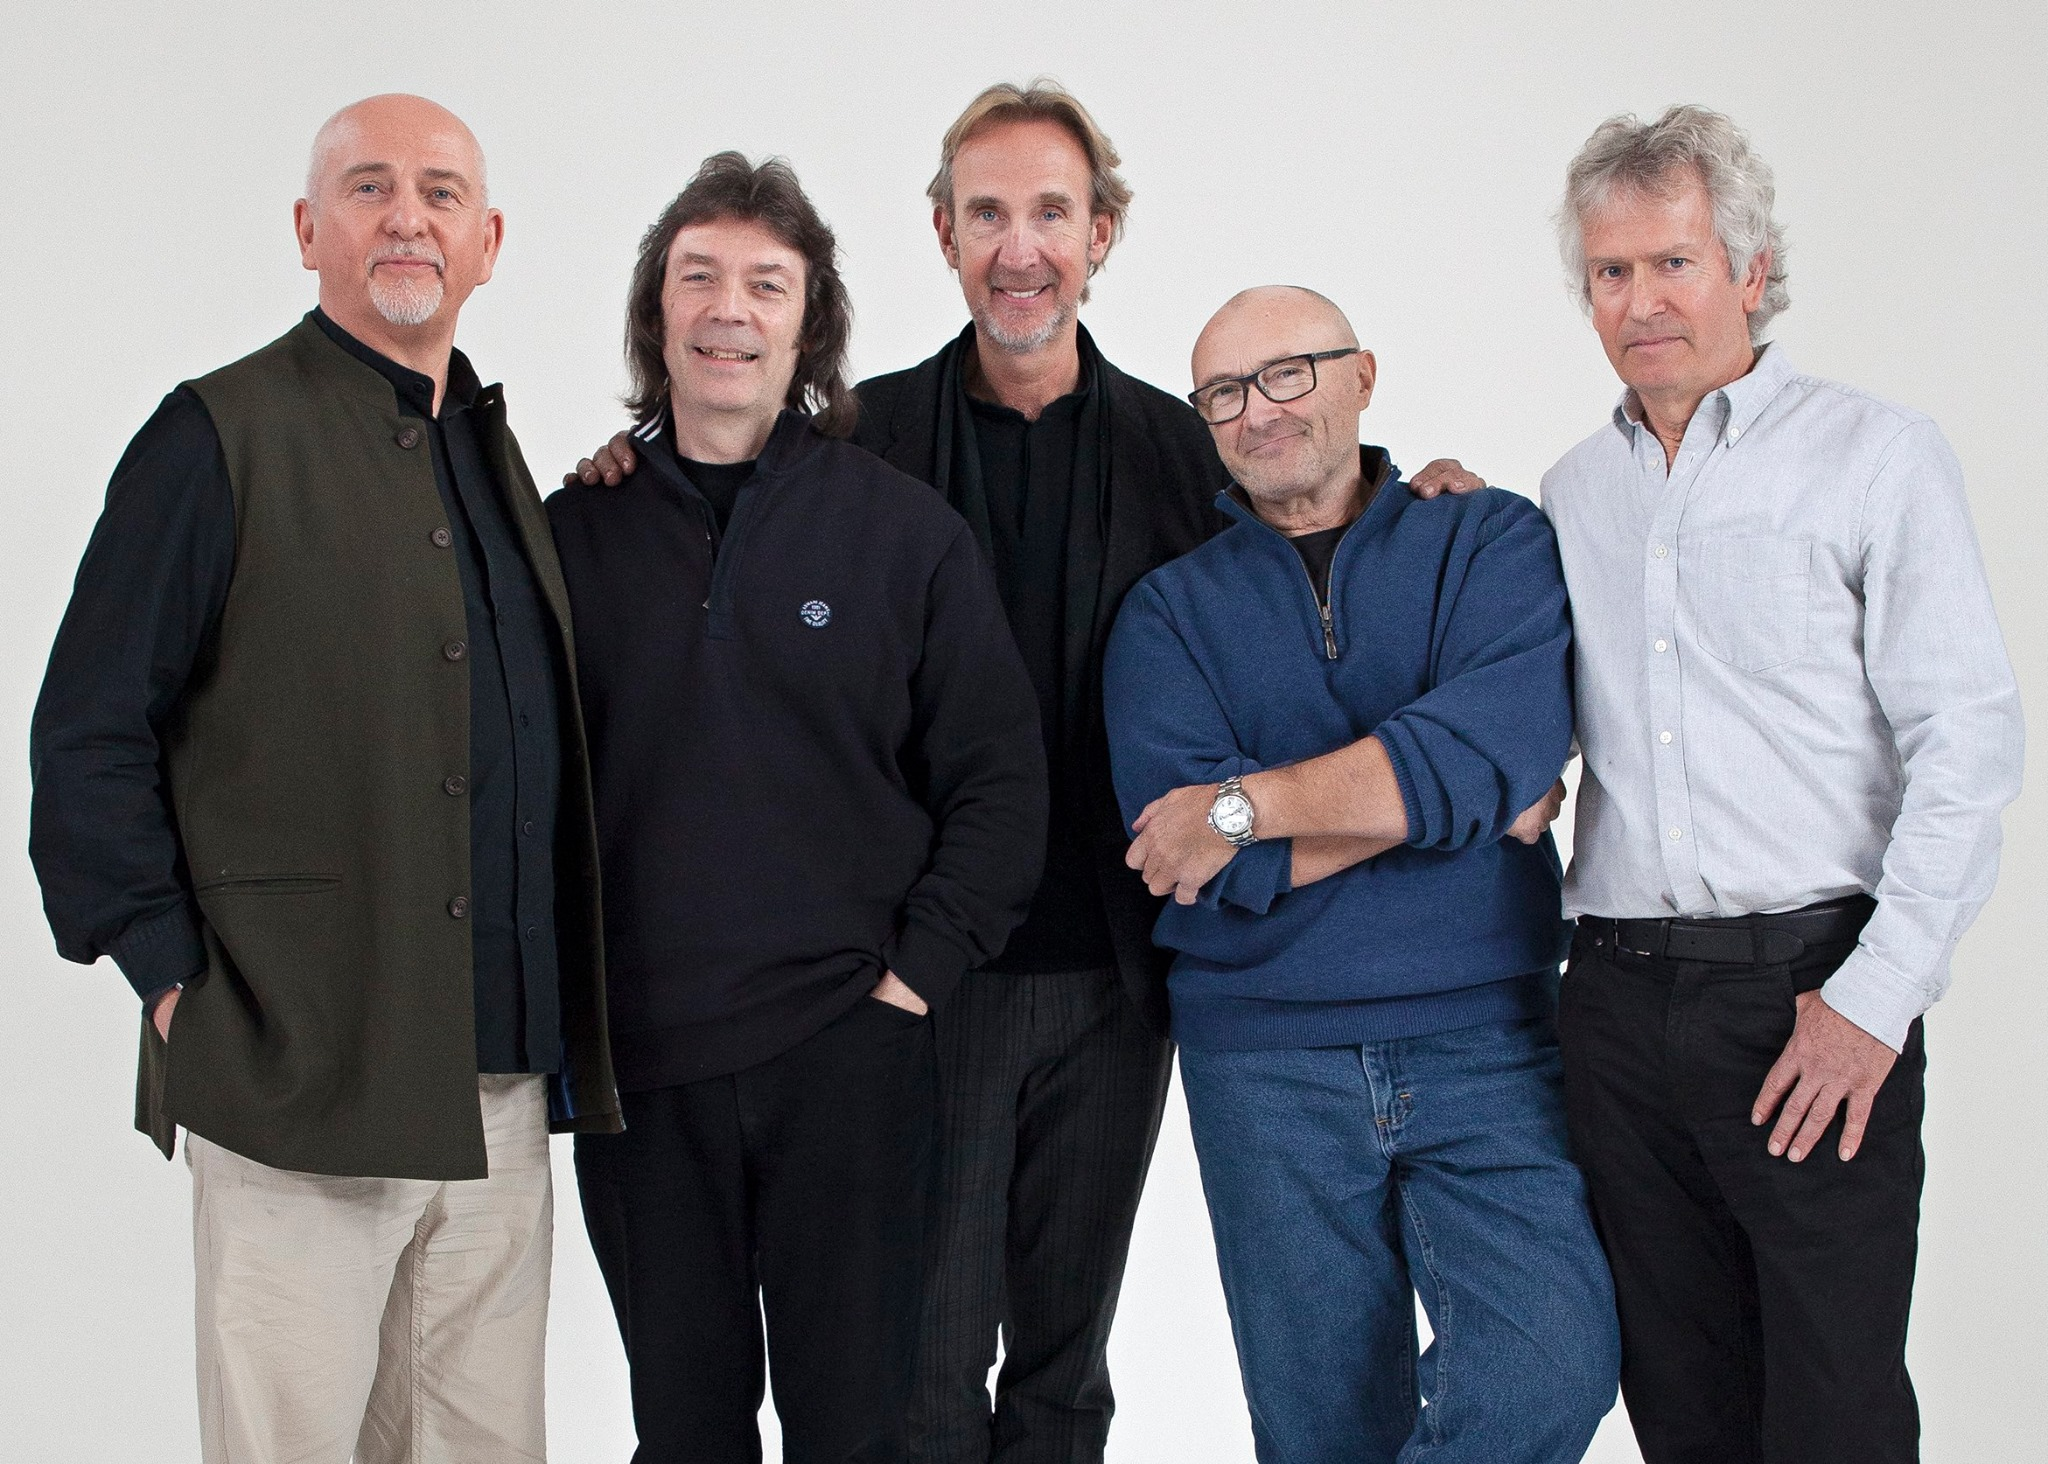
\includegraphics[scale = 0.2]{img/04.jpg}
    \end{center}
    \caption{Phil Collins junto a miembros y ex-miembros de la banda de rock progresivo, Genesis. De izquierda a derecha: Peter Gabriel, Steve Hackett, Mike Rutherford, Phil Collins y Tony Banks.}
  \end{figure}

  %\chapter{Reflexión}

  %\chapter{Conclusiones}

  \bibliographystyle{alpha}
  \bibliography{biblio}
  \addcontentsline{toc}{chapter}{Bibliografía}
\end{document}